\documentclass[10pt,a4paper]{article}
\usepackage[margin=20mm]{geometry}
\usepackage{lmodern}
\usepackage[T1]{fontenc}
\usepackage{graphicx,longtable,booktabs,array,listings}
\usepackage[hidelinks]{hyperref}
\setlength{\emergencystretch}{4em}
\lstset{basicstyle=\ttfamily\scriptsize,breaklines=true,columns=fullflexible}
\title{Public-source generalization pilot}
\author{Five-anomaly evaluation project}
\date{20 October 2026}
\begin{document}\maketitle\tableofcontents\newpage

This is an addendum to the completed 19 October technical runthrough. It records actual new public-data acquisition, 36 classifier fits, new-source SmolVLM transfer, and the full-stream tiling experiment. All measured outputs were produced on the local CUDA runtime without pacing or a latency benchmark. Earlier experiments and their reports are preserved.

\section{Findings and decision}

Full-stream tiling regresses the primary unattended-event result: full-frame detection finds 2/2 published AVSS events with zero reviewed normal-time alerts; both tiled modes find 1/2 and add one normal-time alert. The earlier CAVIAR box-recall gain does not establish a better complete event detector. Retain the full-frame baseline for the next prospective comparison.

The smoking data-addition results are:

\begin{itemize}
\item MobileCLIP, CCTV: old-only to mixed AP 0.6937 to 0.5673; recall 10.2\% to 12.2\%; FPR 5.5\% to 15.8\%.
\item MobileCLIP, XRF55 proxy: old-only to mixed AP 0.4978 to 0.5028; recall 0.0\% to 0.0\%; FPR 0.0\% to 11.1\%.
\item SigLIP2, CCTV: old-only to mixed AP 0.7309 to 0.6227; recall 8.9\% to 36.9\%; FPR 4.0\% to 36.8\%.
\item SigLIP2, XRF55 proxy: old-only to mixed AP 0.3568 to 0.7768; recall 0.0\% to 21.7\%; FPR 0.0\% to 1.7\%.
\end{itemize}
These comparisons use family-specific development-selected heads and frozen development cutoffs. Historical test cohorts have already been inspected in earlier studies. The fresh XRF55 test measures scripted action discrimination on a new scene and three held-out numeric subject groups. It cannot establish improvement on genuine CCTV smoking events. No model is automatically promoted, and no five-objective deployment winner is established.

SmolVLM's original-to-prior-LoRA AP on this proxy source falls from 0.3855 to 0.3573. With newly frozen source-development budget cutoffs, original recall/FPR are 61.7\%/36.7\%; LoRA recall/FPR are 35.0\%/18.3\%. Both older budget cutoffs predict no positives. This is further evidence of scene-dependent ranking and calibration, within the limits of the source-action labels.

\section{Public data collection and label compatibility}

The author XRF55 repository identifies the action mapping and public RGB release. The public Kaggle RGB/depth/IR release, version 6, supplies the selected RGB clips. The release README records CC BY-NC 4.0; retain the source's attribution and use conditions. Local receipts establish downloaded-file identity, not author-issued checksums.

Downloaded: 740 clips, 886,570,077 bytes, representing four publisher primary-action labels: using phone (03), drinking (13), eating (14), smoking (15). There are 185 class-15 clips and 555 controls. Every clip has 75 frames at 15 fps (about five seconds). These short correlated repetitions do not constitute an hour of reviewed normal CCTV exposure.

A visual check restricted to training examples (scene 1, numeric subject 01, actions 03/13/15, frames 10/40/65) found a masked actor and a smoking-labelled hand-to-mouth gesture. A cigarette was not independently verified. The source is therefore retained as a weak smoking-action/gesture proxy. The original class IDs are preserved; no subjective relabelling of held-out examples was used. Publisher primary-action labels are not exhaustive five-anomaly negatives.

{\scriptsize\setlength{\tabcolsep}{3pt}
\begin{longtable}{@{}>{\raggedright\arraybackslash}p{\dimexpr 0.16667\linewidth-6pt\relax}>{\raggedright\arraybackslash}p{\dimexpr 0.16667\linewidth-6pt\relax}>{\raggedright\arraybackslash}p{\dimexpr 0.16667\linewidth-6pt\relax}>{\raggedright\arraybackslash}p{\dimexpr 0.16667\linewidth-6pt\relax}>{\raggedright\arraybackslash}p{\dimexpr 0.16667\linewidth-6pt\relax}>{\raggedright\arraybackslash}p{\dimexpr 0.16667\linewidth-6pt\relax}@{}}
\toprule
Split & Scene IDs & Numeric subject groups & Clips & Positive / controls & Purpose \\
\midrule\endhead
Train & 1 and 2 & 15 (17 scene-subject groups) & 340 & 85 / 255 & Weak supervised fitting \\
Development & 3 & 2 & 160 & 40 / 120 & Selection and cutoffs \\
Test & 4 & 3 & 240 & 60 / 180 & Frozen source transfer \\
\bottomrule\end{longtable}}

Numeric subject IDs are conservatively treated as global aliases across scenes. Train/dev/test aliases do not overlap. Scene IDs denote source blocks; they do not prove distinct cameras. Training uses repetitions 1, 4, 7, 10, 13; development/test use all 20 repetitions. The split supersedes the publisher repetition-only split and was fixed before downloading and model scoring. Test diversity is one scene and three subject groups, regardless of its 240 clips.

Preparation decodes sixteen ordered uniform views (indices rounded across 0--74), resizes to a maximum edge of 768 pixels, and saves JPEG quality 92: 11,840 model-input views. Encoded-file SHA-256 and canonical decoded RGB hashes are saved. No exact decoded pixels cross the new splits or overlap the historical smoking inputs. This does not rule out perceptual similarity or correlated actions within subjects.

Acquisition originally received 404 responses because slashes in individual-file paths were not percent-encoded. The saved transport amendment percent-encodes the entire filename; labels, requested files and splits are unchanged. A separate pre-score amendment aligns ancillary eight-view SmolVLM frame metadata with its selected model inputs.

Other public leads were checked rather than silently counted as new target evidence. PETS original/linked hosts and a CDnet mirror were unavailable during the probes. The AOD survey package already acquired AVSS. One abandoned-luggage repository contained synthetic/Photoshop variants and rendered method outputs; those were rejected as real-event tests. NTU RGB+D's cited taxonomy lacks smoking; Kyoto LMA provides an incompatible depth/skeleton release; the cited bilayer-smoking repository did not supply downloadable annotated clips. The source audit records URLs, observations and exclusions. No independent human reviewer or additional local CCTV was available.

\section{Controlled CLIP smoking experiments}

The two pinned pretrained encoders are frozen: MobileCLIP2-S2 and SigLIP2-B/16-224. This round fits 36 logistic-regression heads, with zero new visual-backbone fine-tunes. Both frozen pretrained encoders and all new features use float32 CUDA, TF32 disabled. The previous six visual CLIP fine-tunes and three SmolVLM LoRA training runs remain separate historical work.

Each encoder has three training families: old-only (2,812 examples), new-only (340 weak proxy clips), mixed (3,152). Each family tries two representations and C in 0.1, 1, 10: 18 candidates per encoder. Logistic regression uses LBFGS, at most 1,000 iterations and tolerance 1e-6; every fitted candidate converged. Weights balance annotated class, source and recording/author group. Exported coefficients and all selection scores are float32.

The full representation concatenates the last view, mean, elementwise maximum and last-minus-first embedding, followed by L2 normalization. Full-plus-crop concatenates normalized full/crop representations and normalizes again. Regions are predicted automatically by the same fixed COCO Faster R-CNN ResNet50 FPN v2 used previously (confidence 0.5, person/backpack/handbag/suitcase); they do not use smoking labels or ground-truth boxes. The highest-confidence contextual person and item regions are combined, with 20\% padding; missing regions fall back to the full image. New data use sixteen views; old samples retain their existing views. This is a clip classifier, not an onset/offset detector.

All candidates use the same combined development cohort of 1,474 cases across four sources. A single global cutoff must yield empirical FPR at most 5\% in each development source. Within each family the selection order is worst-source recall, mean-source recall, worst-source AP, mean-source AP. Both model selections are frozen before held-out scoring. Raw zero and pooled development maximum-F1 cutoffs are also saved.

Because the same combined development set is used, old-only receives new-source calibration and new-only receives old-source development feedback. They differ in classifier training data, not in all forms of source supervision. The new-source test scene and subjects remain held out. The family comparison includes development selection among the same two representations and C values; it does not isolate a single fixed head architecture.

{\scriptsize\setlength{\tabcolsep}{3pt}
\begin{longtable}{@{}>{\raggedright\arraybackslash}p{\dimexpr 0.16667\linewidth-6pt\relax}>{\raggedright\arraybackslash}p{\dimexpr 0.16667\linewidth-6pt\relax}>{\raggedright\arraybackslash}p{\dimexpr 0.16667\linewidth-6pt\relax}>{\raggedright\arraybackslash}p{\dimexpr 0.16667\linewidth-6pt\relax}>{\raggedright\arraybackslash}p{\dimexpr 0.16667\linewidth-6pt\relax}>{\raggedright\arraybackslash}p{\dimexpr 0.16667\linewidth-6pt\relax}@{}}
\toprule
Encoder & Family & Selected representation & C & Train n & Global dev cutoff \\
\midrule\endhead
MobileCLIP & old only & full crop pool a0 & 10 & 2812 & 0.25634 \\
MobileCLIP & new only & full crop pool a0 & 1 & 340 & 0.68169 \\
MobileCLIP & mixed & full pool a0 & 0.1 & 3152 & 0.19145 \\
SigLIP2 & old only & full crop pool a0 & 10 & 2812 & -0.60934 \\
SigLIP2 & new only & full pool a0 & 1 & 340 & 0.40519 \\
SigLIP2 & mixed & full pool a0 & 10 & 3152 & -0.16582 \\
\bottomrule\end{longtable}}

Each encoder scores 1,916 held-out cases: 646 CCTV, 806 Stanford40, 224 Kaggle photos and 240 new-source proxy clips. The first 1,676 are retrospective historical tests; these are not 1,916 independent events or people. Five prediction families per encoder are retained: the three controlled training families, the genuine pretrained contrastive text-margin control, and the frozen historical native strategy.

\subsection{Held-out results at the every-source development budget cutoff}

AP evaluates ranking and does not depend on the displayed cutoff. Recall and FPR use each family's frozen single global development cutoff. TP/P and FP/N make the denominators explicit. A 5\% development constraint is not a guarantee of 5\% test FPR.

{\scriptsize\setlength{\tabcolsep}{3pt}
\begin{longtable}{@{}>{\raggedright\arraybackslash}p{\dimexpr 0.12500\linewidth-6pt\relax}>{\raggedright\arraybackslash}p{\dimexpr 0.12500\linewidth-6pt\relax}>{\raggedright\arraybackslash}p{\dimexpr 0.12500\linewidth-6pt\relax}>{\raggedright\arraybackslash}p{\dimexpr 0.12500\linewidth-6pt\relax}>{\raggedright\arraybackslash}p{\dimexpr 0.12500\linewidth-6pt\relax}>{\raggedright\arraybackslash}p{\dimexpr 0.12500\linewidth-6pt\relax}>{\raggedright\arraybackslash}p{\dimexpr 0.12500\linewidth-6pt\relax}>{\raggedright\arraybackslash}p{\dimexpr 0.12500\linewidth-6pt\relax}@{}}
\toprule
Encoder & Family & Source & n & AP & Recall & FPR & TP/P; FP/N \\
\midrule\endhead
MobileCLIP & old only & Kaggle photos & 224 & 0.9973 & 97.3\% & 3.6\% & 109/112; 4/112 \\
MobileCLIP & old only & CCTV & 646 & 0.6937 & 10.2\% & 5.5\% & 40/393; 14/253 \\
MobileCLIP & old only & Stanford40 & 806 & 0.8802 & 78.6\% & 6.0\% & 110/140; 40/666 \\
MobileCLIP & old only & XRF55 proxy & 240 & 0.4978 & 0.0\% & 0.0\% & 0/60; 0/180 \\
MobileCLIP & new only & Kaggle photos & 224 & 0.4724 & 0.9\% & 0.9\% & 1/112; 1/112 \\
MobileCLIP & new only & CCTV & 646 & 0.6104 & 0.0\% & 0.0\% & 0/393; 0/253 \\
MobileCLIP & new only & Stanford40 & 806 & 0.2457 & 0.0\% & 0.8\% & 0/140; 5/666 \\
MobileCLIP & new only & XRF55 proxy & 240 & 0.4553 & 0.0\% & 0.0\% & 0/60; 0/180 \\
MobileCLIP & mixed & Kaggle photos & 224 & 0.9923 & 95.5\% & 6.2\% & 107/112; 7/112 \\
MobileCLIP & mixed & CCTV & 646 & 0.5673 & 12.2\% & 15.8\% & 48/393; 40/253 \\
MobileCLIP & mixed & Stanford40 & 806 & 0.7915 & 72.1\% & 9.5\% & 101/140; 63/666 \\
MobileCLIP & mixed & XRF55 proxy & 240 & 0.5028 & 0.0\% & 11.1\% & 0/60; 20/180 \\
SigLIP2 & old only & Kaggle photos & 224 & 0.9998 & 99.1\% & 1.8\% & 111/112; 2/112 \\
SigLIP2 & old only & CCTV & 646 & 0.7309 & 8.9\% & 4.0\% & 35/393; 10/253 \\
SigLIP2 & old only & Stanford40 & 806 & 0.9400 & 92.1\% & 8.1\% & 129/140; 54/666 \\
SigLIP2 & old only & XRF55 proxy & 240 & 0.3568 & 0.0\% & 0.0\% & 0/60; 0/180 \\
SigLIP2 & new only & Kaggle photos & 224 & 0.3982 & 0.9\% & 4.5\% & 1/112; 5/112 \\
SigLIP2 & new only & CCTV & 646 & 0.5631 & 0.0\% & 0.4\% & 0/393; 1/253 \\
SigLIP2 & new only & Stanford40 & 806 & 0.2002 & 2.9\% & 2.4\% & 4/140; 16/666 \\
SigLIP2 & new only & XRF55 proxy & 240 & 0.6313 & 61.7\% & 15.6\% & 37/60; 28/180 \\
SigLIP2 & mixed & Kaggle photos & 224 & 0.9982 & 99.1\% & 1.8\% & 111/112; 2/112 \\
SigLIP2 & mixed & CCTV & 646 & 0.6227 & 36.9\% & 36.8\% & 145/393; 93/253 \\
SigLIP2 & mixed & Stanford40 & 806 & 0.9084 & 87.1\% & 7.2\% & 122/140; 48/666 \\
SigLIP2 & mixed & XRF55 proxy & 240 & 0.7768 & 21.7\% & 1.7\% & 13/60; 3/180 \\
\bottomrule\end{longtable}}

\begin{figure}[htbp]\centering
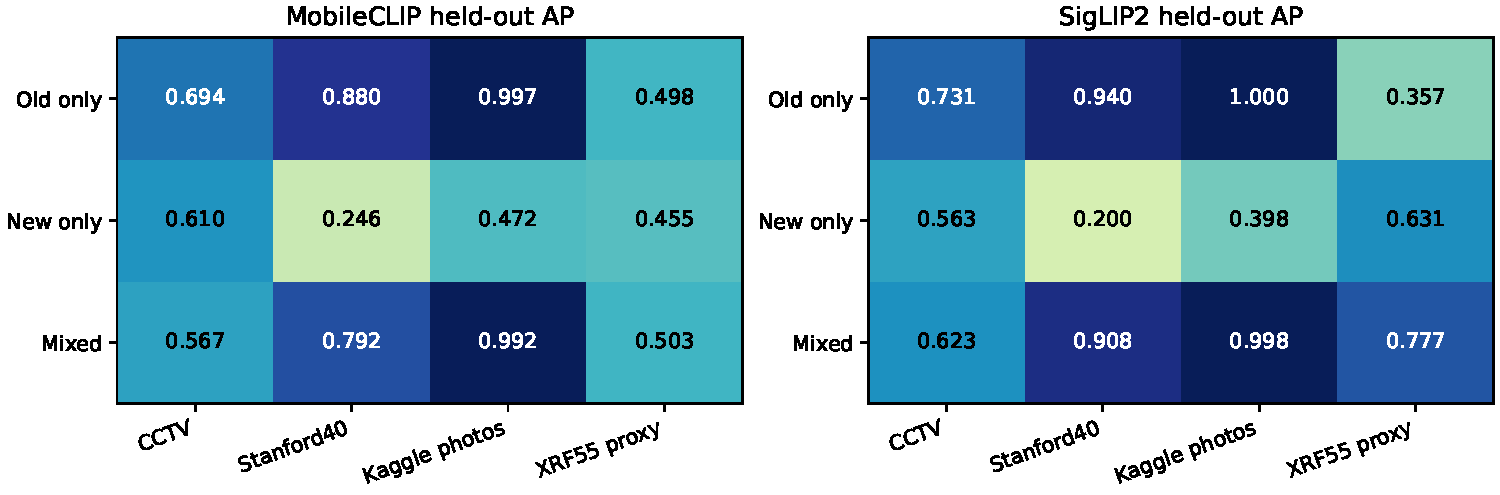
\includegraphics[width=\linewidth]{figures/source_ap.pdf}
\caption{Controlled old/new/mixed held-out ranking by source; historical and fresh proxy evidence remain distinct}
\end{figure}

\subsection{Original and historical reference controls}

The pretrained text score is the mean full-image contrastive binary margin over each clip, with raw zero cutoff. The historical 16 October selected strategy uses its native last-frame smoking input and original development thresholds. It therefore differs from the sixteen-view controlled data-addition recipes. Neither is silently renamed as a newly trained backbone.

{\scriptsize\setlength{\tabcolsep}{3pt}
\begin{longtable}{@{}>{\raggedright\arraybackslash}p{\dimexpr 0.12500\linewidth-6pt\relax}>{\raggedright\arraybackslash}p{\dimexpr 0.12500\linewidth-6pt\relax}>{\raggedright\arraybackslash}p{\dimexpr 0.12500\linewidth-6pt\relax}>{\raggedright\arraybackslash}p{\dimexpr 0.12500\linewidth-6pt\relax}>{\raggedright\arraybackslash}p{\dimexpr 0.12500\linewidth-6pt\relax}>{\raggedright\arraybackslash}p{\dimexpr 0.12500\linewidth-6pt\relax}>{\raggedright\arraybackslash}p{\dimexpr 0.12500\linewidth-6pt\relax}>{\raggedright\arraybackslash}p{\dimexpr 0.12500\linewidth-6pt\relax}@{}}
\toprule
Encoder & Reference & Source & n & AP & Recall & FPR & TP/P; FP/N \\
\midrule\endhead
MobileCLIP & pretrained text & Kaggle photos & 224 & 0.7015 & 81.2\% & 40.2\% & 91/112; 45/112 \\
MobileCLIP & pretrained text & CCTV & 646 & 0.6415 & 1.0\% & 0.8\% & 4/393; 2/253 \\
MobileCLIP & pretrained text & Stanford40 & 806 & 0.2196 & 74.3\% & 63.5\% & 104/140; 423/666 \\
MobileCLIP & pretrained text & XRF55 proxy & 240 & 0.5750 & 96.7\% & 37.2\% & 58/60; 67/180 \\
MobileCLIP & legacy native & Kaggle photos & 224 & 0.9975 & 97.3\% & 3.6\% & 109/112; 4/112 \\
MobileCLIP & legacy native & CCTV & 646 & 0.6902 & 13.5\% & 7.5\% & 53/393; 19/253 \\
MobileCLIP & legacy native & Stanford40 & 806 & 0.8803 & 78.6\% & 6.0\% & 110/140; 40/666 \\
MobileCLIP & legacy native & XRF55 proxy & 240 & 0.4788 & 0.0\% & 0.0\% & 0/60; 0/180 \\
SigLIP2 & pretrained text & Kaggle photos & 224 & 0.8372 & 6.2\% & 0.0\% & 7/112; 0/112 \\
SigLIP2 & pretrained text & CCTV & 646 & 0.6690 & 0.0\% & 0.0\% & 0/393; 0/253 \\
SigLIP2 & pretrained text & Stanford40 & 806 & 0.4994 & 0.7\% & 0.0\% & 1/140; 0/666 \\
SigLIP2 & pretrained text & XRF55 proxy & 240 & 0.5392 & 0.0\% & 0.0\% & 0/60; 0/180 \\
SigLIP2 & legacy native & Kaggle photos & 224 & 0.9998 & 99.1\% & 1.8\% & 111/112; 2/112 \\
SigLIP2 & legacy native & CCTV & 646 & 0.7225 & 4.6\% & 2.4\% & 18/393; 6/253 \\
SigLIP2 & legacy native & Stanford40 & 806 & 0.9373 & 91.4\% & 3.6\% & 128/140; 24/666 \\
SigLIP2 & legacy native & XRF55 proxy & 240 & 0.3498 & 0.0\% & 0.0\% & 0/60; 0/180 \\
\bottomrule\end{longtable}}

All three operating points, all 36 candidate development tables, per-new-subject metrics and per-negative-action prediction rates are preserved in machine-readable outputs. The three-subject test is too small for a strong population-generalization claim; repetition counts must not be treated as independent people.

\subsection{Where the new-source errors occur}

Each action has 60 held-out clips. These are the positive prediction rates at the same frozen development-budget cutoffs. For publisher smoking they represent recall; for the three control actions they represent false-positive proportions within that action, subject to the weak primary-action labels.

{\scriptsize\setlength{\tabcolsep}{3pt}
\begin{longtable}{@{}>{\raggedright\arraybackslash}p{\dimexpr 0.16667\linewidth-6pt\relax}>{\raggedright\arraybackslash}p{\dimexpr 0.16667\linewidth-6pt\relax}>{\raggedright\arraybackslash}p{\dimexpr 0.16667\linewidth-6pt\relax}>{\raggedright\arraybackslash}p{\dimexpr 0.16667\linewidth-6pt\relax}>{\raggedright\arraybackslash}p{\dimexpr 0.16667\linewidth-6pt\relax}>{\raggedright\arraybackslash}p{\dimexpr 0.16667\linewidth-6pt\relax}@{}}
\toprule
Encoder & Family & Smoking & Drinking & Eating & Phone \\
\midrule\endhead
MobileCLIP & old only & 0.0\% & 0.0\% & 0.0\% & 0.0\% \\
MobileCLIP & new only & 0.0\% & 0.0\% & 0.0\% & 0.0\% \\
MobileCLIP & mixed & 0.0\% & 33.3\% & 0.0\% & 0.0\% \\
SigLIP2 & old only & 0.0\% & 0.0\% & 0.0\% & 0.0\% \\
SigLIP2 & new only & 61.7\% & 46.7\% & 0.0\% & 0.0\% \\
SigLIP2 & mixed & 21.7\% & 5.0\% & 0.0\% & 0.0\% \\
\bottomrule\end{longtable}}

All new-source control errors in the controlled CLIP families occur on drinking clips. Mixed SigLIP's per-subject smoking recalls are 10\%, 0\%, and 55\% for numeric aliases 03, 04, and 13; each has 20 positive clips and 60 controls. The aggregate 21.7\% recall therefore conceals large subject variation. These observed error breakdowns are retrospective diagnostics; they do not trigger a new test-fitted threshold or classifier selection.

\section{SmolVLM original-versus-LoRA source transfer}

This is transfer evaluation, with no new SmolVLM training. Compare the pinned original SmolVLM-500M-Instruct against the previous development-selected smoking adapter (seed 42, learning rate 0.0001). The existing adapter changes 4,341,760 language projection parameters; vision remains frozen. No new-source test labels select the adapter or prompt.

Both routes receive the same eight uniformly spaced frames selected from the sixteen-view manifest. The validated native prompt supports up to eight images. This within-SmolVLM comparison is matched; its eight-view input is different from the CLIP sixteen-view recipe. Frozen visual tokens are reused without changing the vision tower. The fixed question includes the existing smoking definition. Scores are the float32 first-answer Yes-minus-No logits, rather than explanations or generated class labels.

Both routes score 160 development cases and freeze new-source maximum-F1 and 5\%-FPR cutoffs before either route scores the 240 test cases. The 19 October original thresholds are retained separately to reveal transfer calibration failure. No fresh-source route substitution is made.

{\scriptsize\setlength{\tabcolsep}{3pt}
\begin{longtable}{@{}>{\raggedright\arraybackslash}p{\dimexpr 0.16667\linewidth-6pt\relax}>{\raggedright\arraybackslash}p{\dimexpr 0.16667\linewidth-6pt\relax}>{\raggedright\arraybackslash}p{\dimexpr 0.16667\linewidth-6pt\relax}>{\raggedright\arraybackslash}p{\dimexpr 0.16667\linewidth-6pt\relax}>{\raggedright\arraybackslash}p{\dimexpr 0.16667\linewidth-6pt\relax}>{\raggedright\arraybackslash}p{\dimexpr 0.16667\linewidth-6pt\relax}@{}}
\toprule
Route & Cutoff calibration & AP & Recall & FPR & TP/P; FP/N \\
\midrule\endhead
original & New-source dev & 0.3855 & 61.7\% & 36.7\% & 37/60; 66/180 \\
original & 19 Oct dev & 0.3855 & 0.0\% & 0.0\% & 0/60; 0/180 \\
lora & New-source dev & 0.3573 & 35.0\% & 18.3\% & 21/60; 33/180 \\
lora & 19 Oct dev & 0.3573 & 0.0\% & 0.0\% & 0/60; 0/180 \\
\bottomrule\end{longtable}}

Native-image inference validates one test case per route against the visual-token cache at an absolute margin tolerance of 0.002. Per-case Yes/No token mass is also retained; a binary margin measures a constrained comparison, not necessarily a confident free-form answer.

\section{Full-stream unattended-item test}

Ten existing recordings are processed from their beginnings to EOF at 2 Hz, with 2,512 unique source images and 12,560 detector views. Seven ABODA videos represent two conservative scene/camera blocks; three AVSS recordings represent one conservative source block. These are three source/camera blocks, not ten independently sampled cameras. All footage was previously inspected. The ABODA intervals remain provisional assistant-derived annotations. Published AVSS EASY/MEDIUM are primary; HARD remains a separate right-censored diagnostic.

The pinned Grounding DINO tiny model uses the unchanged query ``person . bag . backpack . suitcase . cardboard box . package .'', box threshold 0.25 and text threshold 0.20, with maximum item box area 20\% of the full frame. Four 60\%-width/height corner tiles overlap around the center. Coordinates are remapped using actual integer crop offsets and normalized to the full image. Class-wise greedy NMS uses IoU 0.5. Exactly the same raw five views underlie every arm.

\begin{itemize}
\item Full: full-frame people and items only.
\item Item tiles: full-frame people plus full/tiled item proposals; this isolates item proposal coverage.
\item All tiles: full/tiled people and items.
\end{itemize}
Each recording/arm starts with a fresh causal tracker: new confidence 0.25, low confidence 0.20, maximum association gap two seconds, and at least two seconds of owner proximity evidence. The same existing state rule requires known ownership, at least 30 seconds of item stationarity and at least 0.5 seconds of owner absence. Alerts require two seconds persistence, one second release, ten seconds cooldown, and maximum sample gap 1.1 seconds. There is no annotation-driven frame selection, threshold search, state retuning or event-model training in this arm.

The complete recording is processed chronologically without future observations. Event recall uses the first emitted alarm within each positive interval; duplicates are additional alarms within an already detected event. Normal false alerts use only reviewed normal intervals. Positive intervals take precedence at shared boundaries. Alarms during unreviewed time remain unknown, not automatic false positives or correct detections. Alarm delay is measured from annotated event onset, not runtime inference latency.

{\scriptsize\setlength{\tabcolsep}{3pt}
\begin{longtable}{@{}>{\raggedright\arraybackslash}p{\dimexpr 0.14286\linewidth-6pt\relax}>{\raggedright\arraybackslash}p{\dimexpr 0.14286\linewidth-6pt\relax}>{\raggedright\arraybackslash}p{\dimexpr 0.14286\linewidth-6pt\relax}>{\raggedright\arraybackslash}p{\dimexpr 0.14286\linewidth-6pt\relax}>{\raggedright\arraybackslash}p{\dimexpr 0.14286\linewidth-6pt\relax}>{\raggedright\arraybackslash}p{\dimexpr 0.14286\linewidth-6pt\relax}>{\raggedright\arraybackslash}p{\dimexpr 0.14286\linewidth-6pt\relax}@{}}
\toprule
Evidence group & Arm & Detected & Normal FP & Duplicates & Unknown & Normal minutes \\
\midrule\endhead
AVSS censored & full & 1/1 & 0 & 1 & 0 & 1.97 \\
AVSS primary & full & 2/2 & 0 & 0 & 0 & 3.43 \\
ABODA provisional & full & 4/5 & 0 & 0 & 1 & 5.98 \\
AVSS censored & item tiles & 1/1 & 0 & 1 & 0 & 1.97 \\
AVSS primary & item tiles & 1/2 & 1 & 0 & 0 & 3.43 \\
ABODA provisional & item tiles & 2/5 & 0 & 0 & 5 & 5.98 \\
AVSS censored & all tiles & 1/1 & 1 & 1 & 0 & 1.97 \\
AVSS primary & all tiles & 1/2 & 1 & 1 & 0 & 3.43 \\
ABODA provisional & all tiles & 2/5 & 1 & 0 & 4 & 5.98 \\
\bottomrule\end{longtable}}

\begin{figure}[htbp]\centering
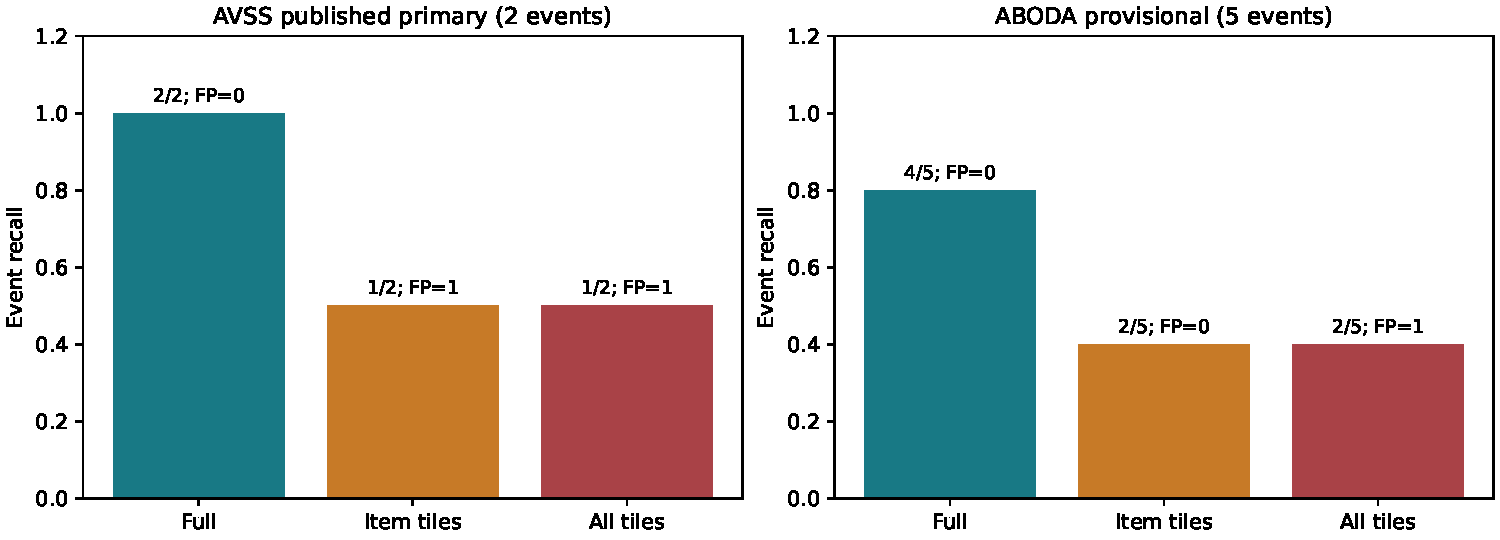
\includegraphics[width=\linewidth]{figures/stream_comparison.pdf}
\caption{Tiling reduces full-stream event recall and introduces normal-time alerts}
\end{figure}

The full-frame primary delays are 24.72 seconds (EASY) and 44.91 seconds (MEDIUM), median 34.82 seconds. The primary normal exposure is 205.739 seconds (3.43 minutes). Zero observed normal alerts yields a one-sided 95\% Poisson upper bound of 52.42 alerts/hour under that rate model; this is far too weak to validate operational reliability. It also does not address camera/domain dependence. HARD's normal exposure is 118.32 seconds and ABODA's is 359 seconds, reported separately.

Earlier primary tables started scoring at t >= 20 seconds, giving 165.739 normal seconds and a 65.07/hour zero-alert bound. Starting at zero adds forty seconds of the same existing recordings, not new cameras or newly collected normal footage. Per-recording aligned t >= 20 metrics are included in results.json for direct comparison. The full-frame arm still detects 2/2 primary events in that aligned exposure.

More proposals are not necessarily better tracks. On MEDIUM, unique emitted item-track IDs increase from 284 (full) to 497 (either tile arm); its event is missed with tiles. On EASY, counts increase from 162 to 371 and a reviewed normal false alarm appears. These are tracker proposal/identity diagnostics, not ground-truth identity-switch rates. They are consistent with more fragmented or spurious associations, but no owner/track reference annotations establish the exact error mechanism. Preserve the failure cases for association and ownership supervision, rather than choosing new rules on these same test recordings.

\section{Verification, artifacts and reproduction}

The stream verifier recomputes all 7,536 tracker/state decisions, every emitted alarm and each per-stream metric from raw detector output; it also checks aggregate counts and 2,512 encoded/decoded image identities. The smoking verifier reconstructs all candidate development scores, cutoffs, convergence flags and all six selected family choices, then reconstructs the selected test and reference scores. It checks all 11,840 new decoded inputs, cross-split aliases/pixels, cache normalization and manifest identity. SmolVLM dev thresholds and test operating points are replayed for both routes.

Native CUDA CLIP validation re-encodes full and crop views for three fixed cases per encoder, covering train/dev/test and both labels, then compares selected head margins against cached features. SmolVLM separately checks its native image path. Verification does not turn weak action labels into verified CCTV truth. The unit suite previously passed 192 tests, including five new tile-coordinate/fusion invariants; test execution output is preserved separately.

Primary local artifacts:

\begin{itemize}
\item data/generalization\_pilot\_20261020/source\_audit.json: public-source decisions and exclusions.
\item data/generalization\_pilot\_20261020/xrf55/: acquisition protocol/amendment, receipts, label audit, manifest, videos, frames and feature caches.
\item results/generalization\_pilot\_20261020/protocol.json, results.json, traces.jsonl, alerts.jsonl: frozen stream settings and all measured arms.
\item results/generalization\_pilot\_20261020/smoking/: shared protocol, all heads, per-candidate dev predictions, frozen selections, test predictions and source/subject/action metrics.
\item results/generalization\_pilot\_20261020/smolvlm\_transfer/: original/adapter protocol, calibration, test predictions, token-cache identities and native-path validation.
\item results/generalization\_pilot\_20261020/verification.json and native\_feature\_validation.json: replay and live CUDA checks.
\item This report's CSVs contain per-stream metrics, aggregate events, all held-out operating points and all development candidates. Figures are supplied as PNG and vector PDF. runthrough.tex is the compilable source for the PDF addendum.
\end{itemize}
Commands and runtime dependencies are in docs/generalization\_pilot.md. The CPU environment handles convex classifier fitting and numerical verification; CUDA handles neural feature extraction and inference. Accuracy runs are unpaced and no new CPU latency experiment is run.

\section{Consequences for the five objectives}

\begin{itemize}
\item Smoking: additional public clips supply an honest weak-label/data-source ablation. Prioritize visible-cigarette confirmation, distant CCTV examples and matched drinking/eating/phone hard negatives. Preserve source separation and a single development-only operating threshold.
\item Unattended items: retain the full-frame causal baseline. The next training target is coherent item/person association, owner evidence and long-gap recovery, with reviewed owner/item histories and longer normal streams. More box recall alone failed this test.
\item Littering: the previous IWDD and transfer evidence remains unchanged in this pilot. Collect or locate independently annotated release/disposal events and matched putting-down/picking-up controls before claiming street-litter generalization.
\item Loitering: previous transfer and seed regressions remain unresolved. Duration, trajectory and scene-zone supervision require longer person tracks and camera/day-separated validation; isolated action clips are insufficient.
\item Rough sleeping: apparent public sleeping/resting remains a visual proxy. Housing status cannot be inferred from appearance. Add independently reviewed temporal resting/wake/movement controls and new locations without broadening the label claim.
\end{itemize}
The next acceptance test should be frozen before any new independent event footage is scored: independent source/camera blocks, explicit onset/offset and owner/item labels where relevant, matched negative exposure, per-source recall/FPR and alert burden with denominators. Under a Poisson model, zero alerts in about three reviewed normal camera-hours gives an upper rate near one/hour; source coverage and a longer observation period are still needed. Neither 740 repeated lab clips nor 3.43 minutes of primary normal video solves that evidence gap.
\end{document}
